%!TEX root = ../thesis.tex
\section{Authoring}
% \section{Recording with Kinectograph}
%\bjoern{moved to intro}Kinectograph serves as both the camera and the cameraman. It provides a motorized dock for a Kinect sensor and a tablet-based user interface (separate from the camera) to control the camera orientation (Figure 1). By using the Kinect to track the user’s movement, Kinectograph automatically pans and tilts the camera in real time. The portable size of Kinectograph makes it easy to be placed on a tabletop surface or a TV stand to capture the room where the user will perform.

\begin{figure}[t]
\centering
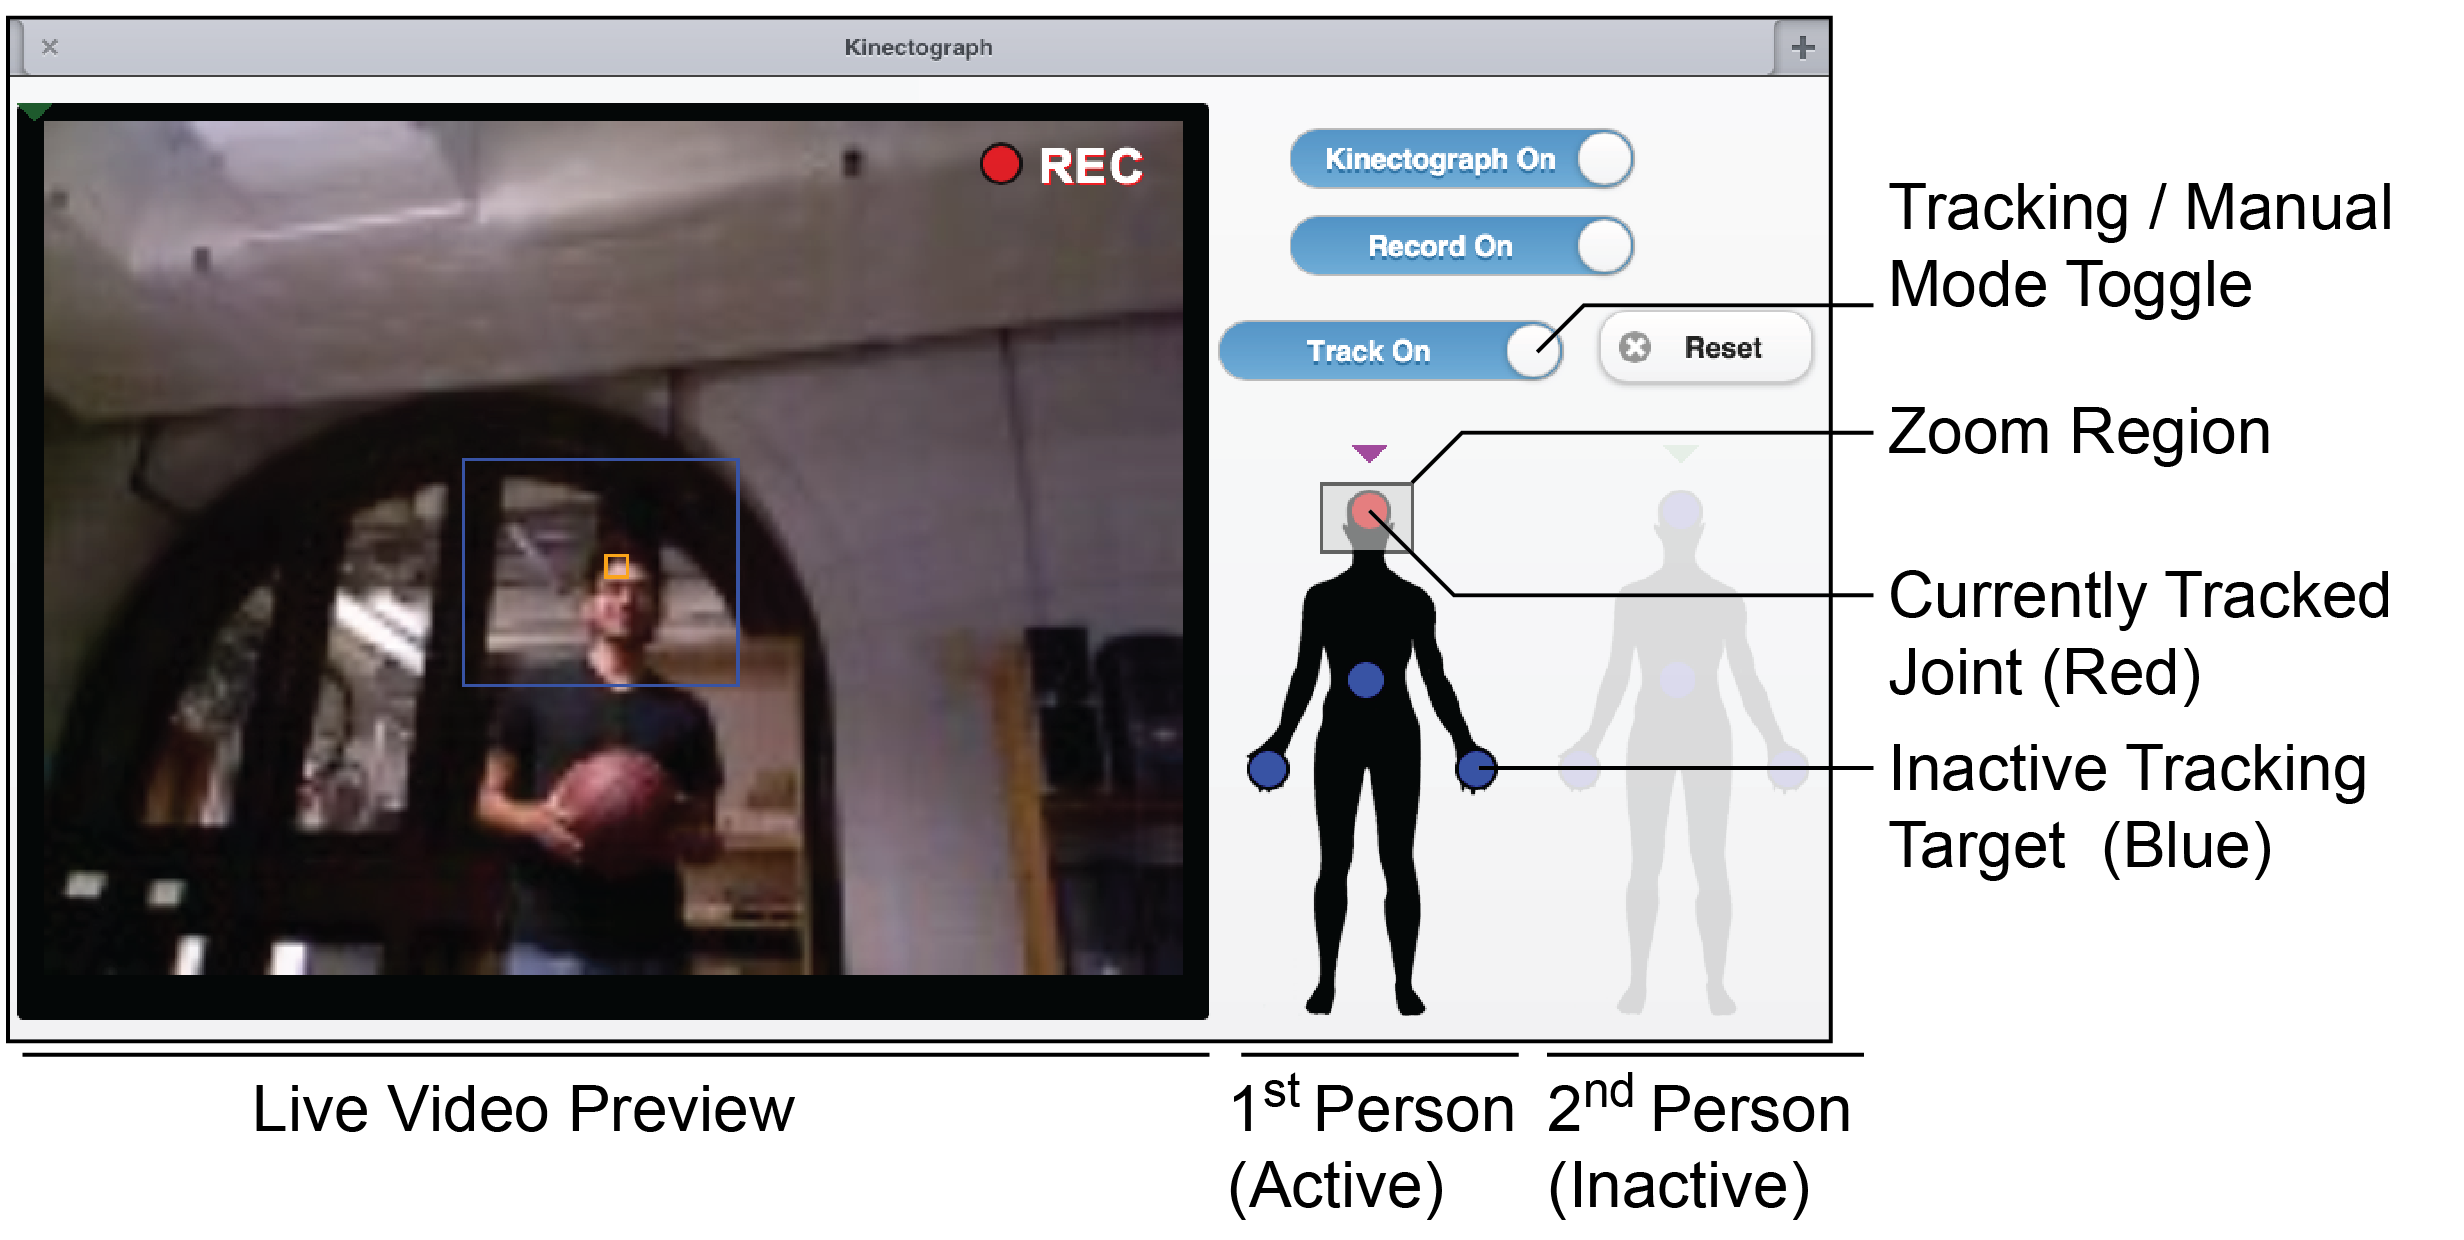
\includegraphics[width=1.0\columnwidth]{\kinectograph/fig/newui}
\caption{Kinectograph UI on a tablet device}
\label{fig:figure4}
\end{figure}

Users connect the Kinectograph device to a personal computer and start its server software, then open the Kinectograph mobile control UI (Figure \ref{fig:figure4}) on a phone or tablet that they can carry with them during their demonstration.
% \bh{You had an architecture figure at some point. Where did it go?}
%
In order to allow How-To tutorial makers as much control over the filming of their tutorial with as little effort as possible, Kinectograph offers the following features on its mobile control UI:

\subsection{Real-time Video View}
In a self video recording, it is convenient for the user to be able to view the current state of their video to make filming decisions. Thus, Kinectograph's UI displays a real-time video feed (currently limited to a low fps) from the Kinect camera.

\subsection{Manual Control}
Users can manually control the camera angle by swiping on the preview image to pan and tilt the camera. For example, during a cooking demonstration, users may wish to pan to a shot of the oven to their left or the sink to their right, or tilt down when they open the oven.
% We share this interaction technique with robotic telepresence systems (e.g. Revolve Robotics' Kubi \footnote{http://www.revolverobotics.com/}). %\bh {does zoom work in manual mode? I don't know how.}

\subsection{Automated Tracking Control}
Demonstrations may require users to move around, such as in furniture assembling or personal training videos. Kinectograph's automated tracking control enables users to focus on their demonstration. Thus, users can switch to automatic camera mode to have Kinectograph track them. Kinectograph can follow one or two actors. Users select which body parts should remain in the frame by tapping on targets of an iconic body outline in the UI - e.g., the head (as in video conferencing systems) or the hands (which may be more important for demonstrations). To keep the entire upper body in view, users can select multiple joints simultaneously. Each selected joint can be deselected by toggling the target button on the iconic body outline.

Early testing showed that because the video feed to the tablet has some latency and a lower framerate, selecting joints on the video feed itself can be difficult if those joints are moving. We therefore chose to display a static, iconic body outline.
%display an iconic body outline next to the video feed on the UI to give users a static target for activating and deactivating joint tracking.

%An indicator marker is overlaid on the realtime view to show where where the camera will center (e.g., if multiple joints are tracked, the center of those joints will be displayed). \bjoern{don't need this i think}

\subsection{Zoom Control}
Close-ups of important steps are a common editing technique in demonstration videos. To capture close-ups, users can define a zoom region related to their body by dragging a rectangular area across the iconic body outline - e.g., they can draw a region that captures their hands to focus on their hand motions. Because the camera used has a fixed focal length, our current prototype uses digital zoom (Figure~\ref{fig:ZoomView}). By default any joints in the zoomed region are automatically added to the track list.

\subsection{Reset}
Finally, the UI provides a button to dismiss any joints selected for automated tracking or for zooming.

\begin{figure}[t]
\centering
\includegraphics[width=1\columnwidth]{\kinectograph/fig/ZoomView}
\caption{Kinectograph tracks and provides a digital zoom view (right) captured from the Kinect camera view (left) in real-time based on user specified area.}
\label{fig:ZoomView}
\end{figure}

\begin{figure}[t]
\centering
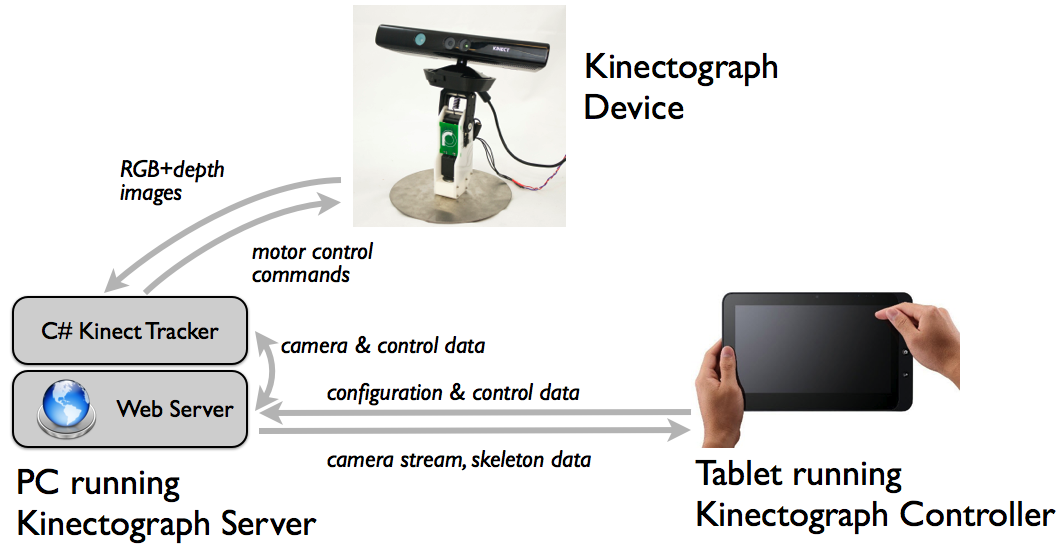
\includegraphics[width=1.0\columnwidth]{\kinectograph/fig/arch.png}
\caption{Kinectograph Architecture}
\label{fig:architecture}
\end{figure}
